\documentclass{article}
\title{Blanchard Ch.16}
\author{Dawei Wang}
\date{\today}
\usepackage{ctex}
\usepackage{amsmath}
\usepackage{amssymb}
\usepackage{graphicx} %插入图片的宏包
\usepackage{float} %设置图片浮动位置的宏包
\usepackage{subfigure} %插入多图时用子图显示的宏包
\begin{document}
	\maketitle

\section{预期和决策}

\subsection{预期、消费和投资决策}

\begin{figure}[H] %H为当前位置,!htb为忽略美学标准,htbp为浮动图形
	\centering %图片居中
	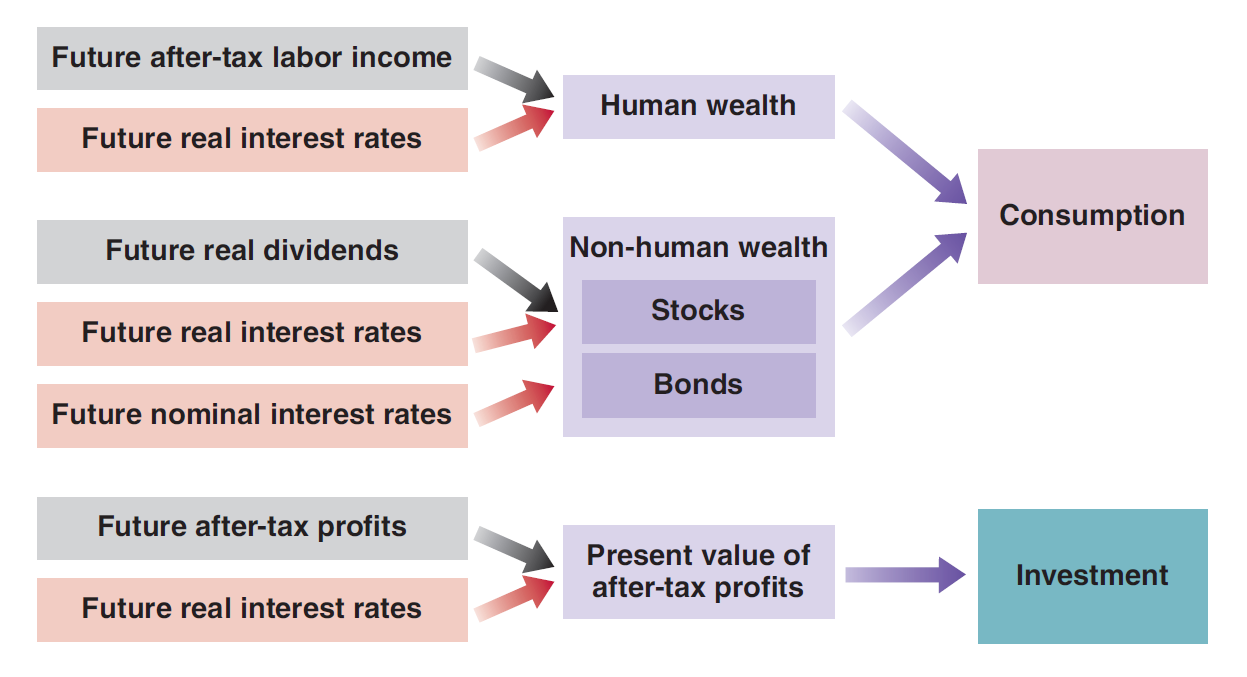
\includegraphics[width=1\textwidth]{16_1} %插入图片,[]中设置图片大小,{}中是图片文件名
	\caption{Expectations and Private
		Spending: The Channels} %最终文档中希望显示的图片标题
	\label{Fig.main2} %用于文内引用的标签
\end{figure}

未来的预期变量通过许多渠道影响当前决策,它通过资产价格直接影响决策的制定。

当前和预期未来的税后实际劳动收入提高,或者当前和预期未来的实际利率降低,则人力财富会增加(税后劳动实际收入的预期现值),从而使消费增加。

当前和预期未来实际红利提高,或者当前和预期未来实际利率降低,会使股票价格提高,从而带来非人力财富的上升,使消费增加。

当前和预期未来的名义利率下降会带来债券价格的上升,从而使非人力财富和消费增加。(这种情况下,债券的名义值比实际值重要,因为债券是在未来对美元有索取权,而非对产品。)

\subsection{预期和IS关系}

将现在和将来缩减成为两个时期:1.当前时期;2.未来的时期。

当前时期的IS关系:

\[
Y=C(Y-T)+I(Y,r+x)+G
\]

加预期修正后的形式:

\[
A(Y,T,r,x)\equiv C(Y-T)+I(Y,r+x)
\]

A代表私人总支出(aggregate private spending),或者简单地说,私人支出(private spending)。

因此IS关系可以改写为:

\[
Y=A(Y,T,r,x)+G
\]

私人总支出是收入的增函数,是税收、实际政策利率和风险溢价的减函数。

\hspace*{\fill}

假设风险溢价是一个常数,若关注预期,对上式的拓展不仅取决于当前变量,还取决于未来的预期值。

\[
Y=A(Y,T,r,Y'^e,T'^e,r'^e)+G
\]

$ Y'^e $、$ T'^e $、$ r'^e $分别表示未来预期收入、未来预期税收和未来预期实际利率。

当期或者未来收入的增加会使私人支出提高;

当期或者未来税收的增加会使私人支出减少;

当期或者未来实际利率的增加会使私人支出减少。

\begin{figure}[H] %H为当前位置,!htb为忽略美学标准,htbp为浮动图形
	\centering %图片居中
	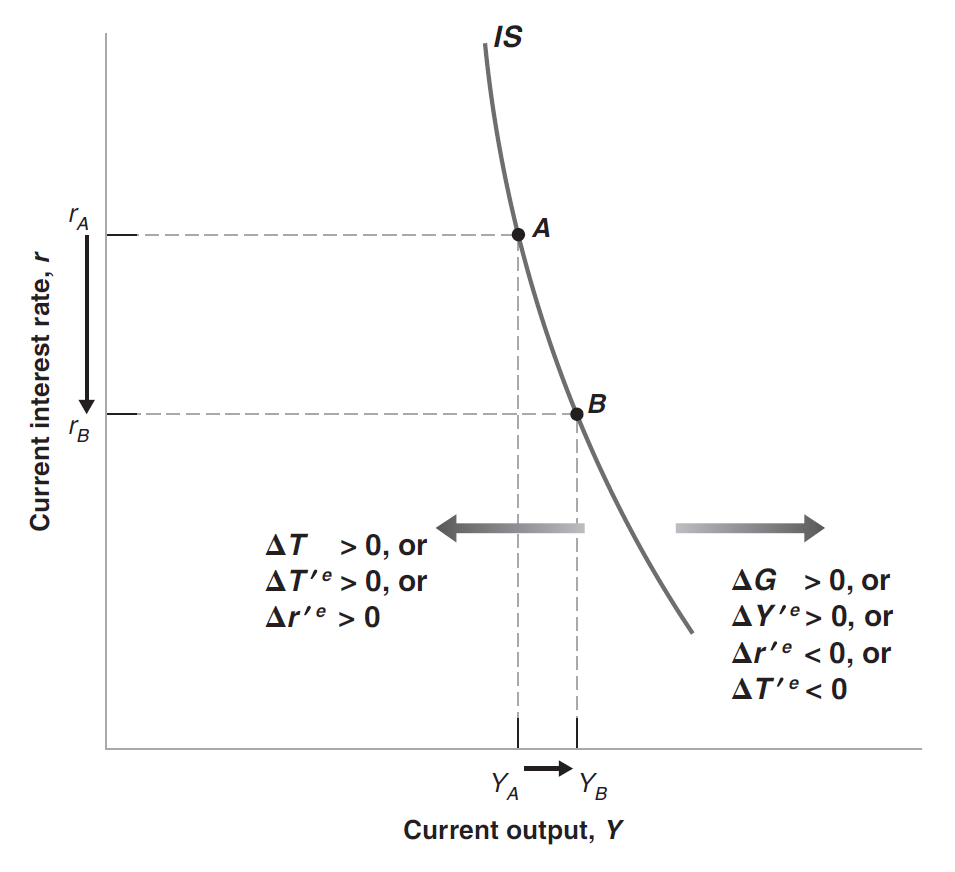
\includegraphics[width=1\textwidth]{16_2} %插入图片,[]中设置图片大小,{}中是图片文件名
	\caption{The New IS Curve} %最终文档中希望显示的图片标题
	\label{Fig.main3} %用于文内引用的标签
\end{figure}

设定除当前产出Y和当前实际政策利率r之外的一切变量都是给定的。因此,IS曲线是在给定当前和未来的预期税收T和$ T'^e $、预期产出值$ Y'^e $以及未来实际政策利率$ r'^e $的情况下画出。

新的IS曲线依旧向下倾斜,当前实际政策利率的下降导致支出上升。支出的上升通过乘数效应导致产出上升。新的IS曲线比之前的IS曲线更加陡峭:在其他情况保持不变的条件下,当前政策利率大幅度下降可能只对产出有很小的影响。

\hspace*{\fill}

利率对产出的影响取决于两种效应的强度: 给定收入的情况下实际利率对支出的影响;以及乘数效应的大小。

在未来实际利率的预期保持不变的情况下,当前实际利率的下降不会对支出产生很大影响。当前实际利率的变化不会使现值发生很大变化,从而也不会使支出发生很大变化。

乘数效应可能很小。乘数效应的大小取决于当前收入变化对支出影响的大小。但是,在未来收入预期保持不变的情况下,当前收入的变化不会对支出产生很大影响。原因是:一个预期不会持续很久的收入变化对消费和投资的影响是有限的。

当前税收T,或者当前政府支出G的变化会使IS曲线移动;

预期未来变量$ (Y'^e,T'^e,r'^e) $的变化也会使IS曲线发生移动。

\section{货币政策、预期和产出}

\begin{figure}[H] %H为当前位置,!htb为忽略美学标准,htbp为浮动图形
	\centering %图片居中
	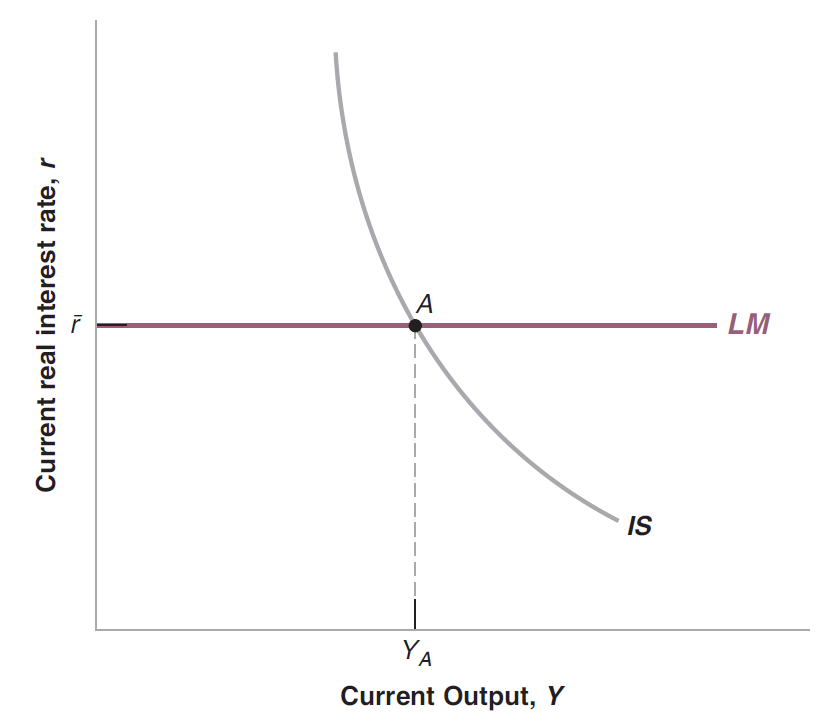
\includegraphics[width=1\textwidth]{16_3} %插入图片,[]中设置图片大小,{}中是图片文件名
	\caption{The New IS-LM} %最终文档中希望显示的图片标题
	\label{Fig.main4} %用于文内引用的标签
\end{figure}

\[
IS:\enspace Y=A(Y,T,r,Y'^e,T'e,r'e)+G
\]

\[
LM:\enspace r=\overline{r}
\]

美联储会直接影响到的利率是当前实际利率r,因此,LM曲线依然是一条水平线,其值等于美联储给定的实际政策利率$ \overline{r} $。

\subsection{重新审视货币政策}

给定预期时,货币供给的增加导致LM曲线发生移动,并沿着陡峭的IS曲线向下变动,结果是r大幅下降而Y小幅增加。

\begin{figure}[H] %H为当前位置,!htb为忽略美学标准,htbp为浮动图形
	\centering %图片居中
	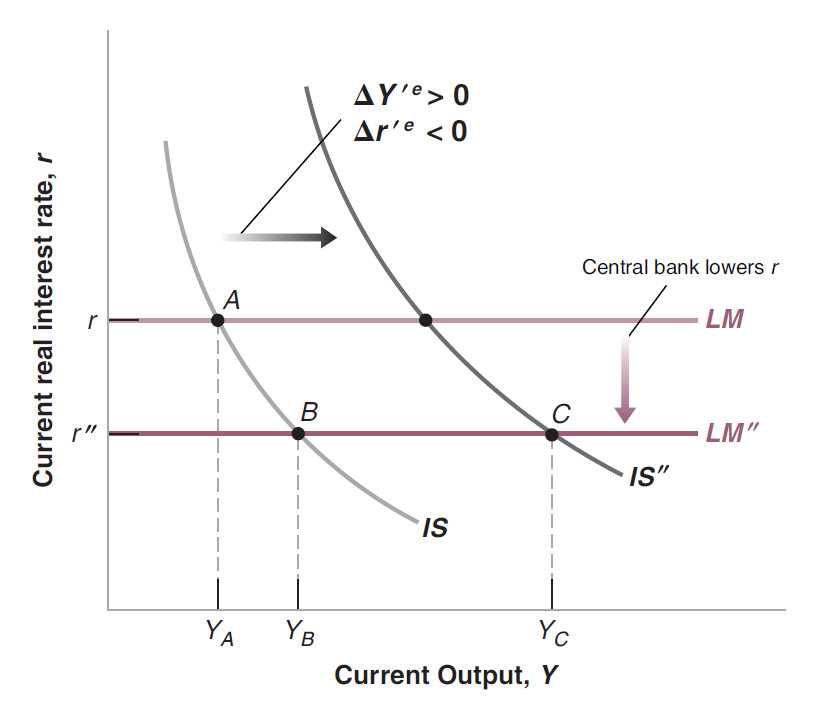
\includegraphics[width=1\textwidth]{16_4} %插入图片,[]中设置图片大小,{}中是图片文件名
	\caption{The Effects of an
		Expansionary Monetary
		Policy} %最终文档中希望显示的图片标题
	\label{Fig.main5} %用于文内引用的标签
\end{figure}

考虑预期的影响,给定当前利率,预期未来利率更低和未来产出更高都会使支出和产出更高,它们使IS曲线向右移动,从IS移动至IS''。新的均衡点处于C点。因此,即使扩张性货币政策对产出的直接影响是有限的,但一旦考虑预期的变化,其总影响很大。

任何一种宏观经济政策的效果,都极大依赖于预期的效应。

如果扩张性的货币政策使金融投资者、公司以及消费者改变了对未来利率和未来产出的预期,那么该政策对产出的影响可能非常大。

如果预期保持不变,那么扩张性货币政策对产出的影响会比较小。

我们说某一政策的作用取决于预期的影响,并不是说任何事情都会发生,预期不是任意的。

建立在前沿方式上的预期称作理性预期(rational expectations)。

\hspace*{\fill}

考虑预期的两种方法:

“动物精神”:来自凯恩斯的《通论》,认为预期的变动被认为是重要的,但无法解释。

“向后看规则”:静态预期(static expectations),也就是说,像现在那样去预期未来。或者假定人们有适应性预期(adaptive expectations),例如,在给定时间给定变量的条件下,人们的预期被证实过低,那么他们会在接下来的时期内提高该变量的预期值以适应变量的变化。

\section{减少赤字、预期和产出}

在短期,除非假设未来产出的预期$ Y'^e $和未来利率的预期$ r'^e $保持不变。此时当前时期政府支出的减少导致IS曲线向左移动,使均衡产出降低。

在中期,赤字削减对产出没有影响,但是它带来更低的利率和更高的投资。

在中期,自然产出水平取决于生产水平以及就业的自然水平。自然就业水平取决于自然失业水平。如果政府在产品市场和劳务市场的支出并没有影响自然失业率,而且并没有明显的理由能说明这会有影响,那么支出的变动将不会影响自然产出水平。因此,赤字缩减在中期不会对产出水平有影响。

现在考虑产出必然等于支出,以及支出是公共支出和私人支出之和。给定产出水平不变,当公共支出降低时,私人支出必然会提高。更高的私人支出要求更低的利率。低利率导致更高的投资,因而有更高的私人支出,这才能抵消公共支出的下降,从而使产出保持不变。

\hspace*{\fill}

在长期,即考虑资本积累对产出的影响,更高的投资导致更高的资本存量,从而导致更高的产出。

产出中用于储蓄的比例越高,资本存量越高,因而长期内的产出水平越高。

将未来时期看着包含中期和长期。如果个人、公司和金融市场参与者有理性预期,那么他们对于宣布赤字缩减反应是预期未来会发生这些变化。因此,他们预期未来产出$ Y'^e $提高,未来利率$ r'^e $下降。股票价格上涨,人们知悉这些预测并观察债券和股票价格,将会调整他们的支出计划以增加支出。

\hspace*{\fill}

在中期:产出Y并未发生变化,而投资提高。

在长期:I增加$ \Rightarrow $K增加$ \Rightarrow $Y增加。


\subsection{回到当前时期}

对于宣布赤字缩减的反应,现在有三个因素使IS曲线发生变动:

\begin{figure}[H] %H为当前位置,!htb为忽略美学标准,htbp为浮动图形
	\centering %图片居中
	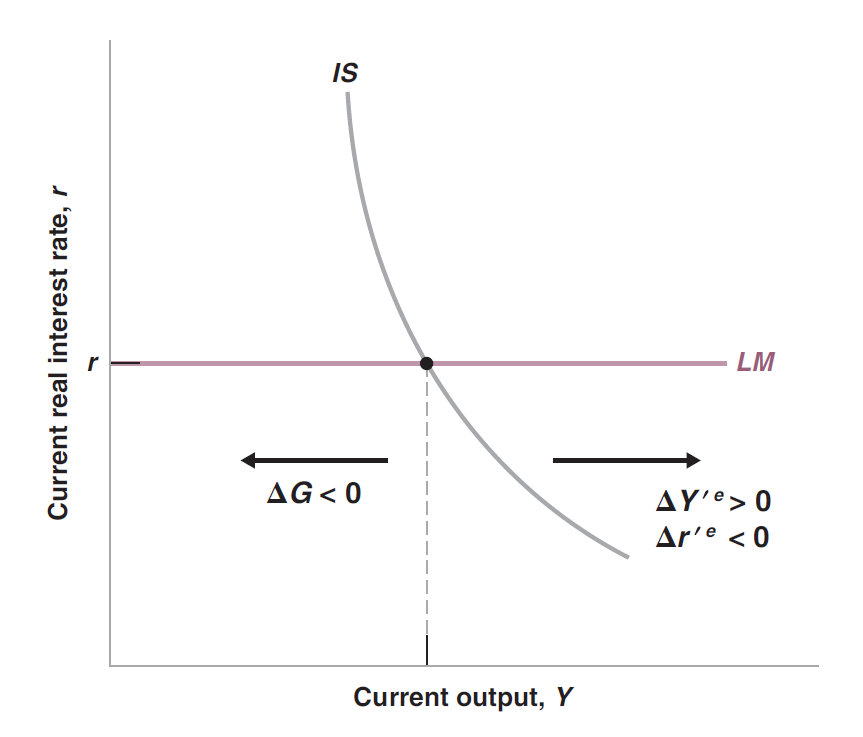
\includegraphics[width=1\textwidth]{16_5} %插入图片,[]中设置图片大小,{}中是图片文件名
	\caption{The Effects of a Deficit
		Reduction on Current
		Output} %最终文档中希望显示的图片标题
	\label{Fig.main6} %用于文内引用的标签
\end{figure}


当前政府支出G下降,导致IS曲线向左移动。在给定利率的条件下,政府支出的下降导致总支出的下降,从而产出下降。

预期未来产出$ Y'^e $提高,导致IS曲线向右移动。在利率给定的条件下。预期未来产出的增加使私人支出上升,从而提高产出。

预期未来利率$ r'^e $下降,导致IS曲线向右移动。在当前利率给定的条件下,未来利率的下降会刺激支出,从而提高产量。

\hspace*{\fill}

对应赤字的缩减,产出可能会上升,也可能会下降。

时机问题:当前政府支出G的下降幅度越小,对当前支出的副作用越小。同时预期未来政府支出的下降幅度越大,对于预期未来产出和利率的影响越大,从而对当前支出的正面影响越大。这意味着将赤字缩减计划延迟至未来,即当前的缩减小一些,而未来的缩减变大更有可能使产出增加。但政府的赤字缩减计划延迟会使计划的信用水平(credibility)降低。

内容问题:赤字的减少有多少是由于税收的提高,有多少是由于支出的减少,这是比较重要的一个问题。如果政府支出项目被认定为不必要,今天把这些项目砍掉可以使政府在未来减少税费。未来税费减少和动乱减少的预期使政府能在今天投资,因此短期内可以提高产出。

初始状况问题:如果经济体中的政府无法有效地控制预算,政府支出很高,税收收入降低,从而赤字很大,那么政府债务会快速增长。这样一个环境下,一个可信的赤字削减计划也很有可能在短期内提高产出。

货币政策问题:货币政策可以通过降低政策利率来减少其对产出的负面影响。

\hspace*{\fill}

总结:赤字削减计划在短期内也可以提高产出,它取决于许多因素,如:

计划的信用、计划的内容、政府的初始财务状况、货币和其它政策。

财政乘数:把直接和预期效应考虑进去后财政整合的净效应。

























 














\end{document}